\section* {3.1}

\subsection{Постановка задачи}
Используя таблицу значений $Y_i$  функции $y=f(x)$, вычисленных в точках   $X_i, i=0,..3$  построить интерполяционные многочлены Лагранжа и Ньютона, проходящие через точки $\{X_i,Y_i \}$ .  Вычислить значение погрешности интерполяции в точке $X^*$. 

{\bfseries Вариант:} 28

y=x*cos(x), а)Xi=[0,pi/6,2pi/6,3pi/6], б)Xi=[0,pi/6,5pi/12,pi/2], x*=pi/4
%\pagebreak

\subsection{Результаты работы}
\begin{figure}[h!]
\centering
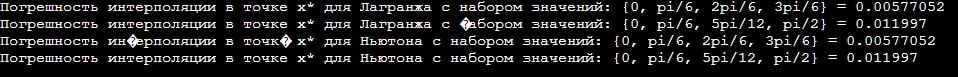
\includegraphics[width=12cm, height=6.5cm]{img/img1}
\caption{Вывод программы в консоли}
\end{figure}
\pagebreak
% \vfill

\subsection{Исходный код}

\lstinputlisting{include/task_1.cpp}
\pagebreak

\section* {3.2}

\subsection{Постановка задачи}
Построить кубический сплайн для функции, заданной в узлах интерполяции, предполагая, что сплайн имеет нулевую кривизну при $x=x_0$  и $x=x_4$. Вычислить значение функции в точке $x=X^*$. 

{\bfseries Вариант:} 28
(f(xi), xi): [(0, 0),(1, 0.45345),(2, 0.52360),(1, 2.7183),(2, 14.778)]
%\pagebreak

\subsection{Результаты работы}
\begin{figure}[h!]
\centering

\includegraphics[width=15cm, height=3cm]{img/img2_2}
\caption{Вывод программы в консоли}
\end{figure}
\pagebreak

\subsection{Исходный код}

\lstinputlisting{include/task_2.cpp}
\pagebreak

\section* {3.3}

\subsection{Постановка задачи}
Для таблично заданной функции путем решения нормальной системы МНК найти приближающие многочлены a) 1-ой  и б) 2-ой степени. Для каждого из приближающих многочленов вычислить сумму квадратов ошибок. Построить графики приближаемой функции и приближающих многочленов.

{\bfseries Вариант:} 28
(xi,f(xi)): [(-1.7, 0.52796),(-1.2, 0.43372),(-0.7, 0.24333),(-0.2, 0.03275),(0.3, 0.12149),(0.8, 1.4243)]
%\pagebreak

\subsection{Результаты работы}
\begin{figure}[h!]
\centering
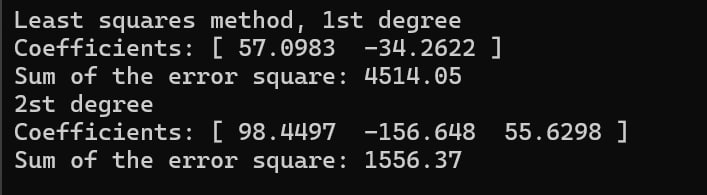
\includegraphics[width=15cm, height=4cm]{img/img3_2}
\caption{Вывод программы в консоли}
\end{figure}
\pagebreak

\subsection{Исходный код}
\lstinputlisting{include/task_3.cpp}
\pagebreak

\section* {3.4}

\subsection{Постановка задачи}
Вычислить первую и вторую производную от таблично заданной функции $y_i=f(x_i), i=0,1,2,3,4$  в точке $x=X_i$.   

{\bfseries Вариант:} 28
Вычислить первую и вторую производную от таблично заданной функции yi=f(xi) в точке x=x*. Входные данные: таблица пар типа (xi,f(xi)): [(0, 0),(0.2, 0.048856),(0.4, 0.23869),(0.6, 0.65596),(0.8, 1.4243)], x*=0.4
%\pagebreak

\subsection{Результаты работы}
\begin{figure}[h!]
\centering
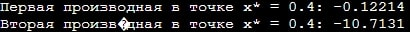
\includegraphics[width=10cm, height=2cm]{img/img4}
\caption{Вывод программы в консоли}
\end{figure}
\pagebreak

\subsection{Исходный код}

\lstinputlisting{include/task_4.cpp}
\pagebreak
\section* {3.5}

\subsection{Постановка задачи}
Вычислить определенный интеграл $\int\limits_{X_0}^{X_1} y dx$  , методами прямоугольников, трапеций, Симпсона с шагами $h_1,h_2$. Оценить погрешность вычислений, используя  Метод Рунге-Ромберга: 

{\bfseries Вариант:} 26\\
y=x^3 -4+x^2, x0=1, xk=5, h1=1, h2=0.5

\subsection{Результаты работы}
\begin{figure}[h!]
\centering
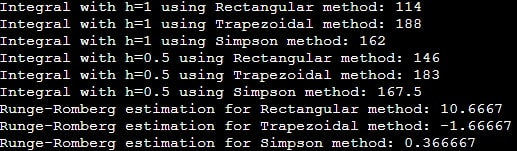
\includegraphics[width=10cm, height=10cm]{img/img5}
\caption{Вывод программы в консоли}
\end{figure}
\pagebreak


\subsection{Исходный код}
\lstinputlisting{include/task_5.cpp}

